\documentclass[letterpaper,journal,transmag]{IEEEtran}

\usepackage{ucs}
\usepackage[spanish]{babel}
\usepackage[utf8x]{inputenc}
\usepackage{amsmath}
\usepackage{amsfonts}
\usepackage{amssymb}
\usepackage{amsthm}
\usepackage{fontenc}
\usepackage{graphicx}

\usepackage{pstricks}
\usepackage{pspicture}
\usepackage{tikz}
\usepackage{pst-text, pst-grad}
\usepackage{hyperref}

\usepackage{multicol}

\usepackage{fancyhdr}


\graphicspath{{./}{./fig/}}
\hyphenation{op-tical net-works semi-conduc-tor}


\begin{document}
%
% paper title
% can use linebreaks \\ within to get better formatting as desired
% Do not put math or special symbols in the title.
\title{Mano robótica}


% author names and affiliations
% transmag papers use the long conference author name format.

\author{\IEEEauthorblockN{David Díaz Barquero}
\IEEEauthorblockA{Área de Ingeniería en Computadores, Tecnológico de Costa
Rica, Cartago, Costa Rica}
}



% The paper headers
\markboth{Junio~2014}%
%%%\markboth{Journal of \LaTeX\ Class Files,~Vol.~11, No.~4, December~2012}%
{Shell \MakeLowercase{\textit{et al.}}: Bare Demo of IEEEtran.cls for Journals}



\IEEEtitleabstractindextext{%
\begin{abstract}
Se desarrollan varios controles para el control de una mano robótica, se decide
utilizar la desarrollada por Langevin. Utilizando un Leap Motion se imita
directamente los movimientos de la mano de una persona, logrando mover
individualmente cada dedo o varios de manera simultánea y un Emotiv para abrir
y cerrar todos los dedos utilizando procesos mentales.
\end{abstract}

% Note that keywords are not normally used for peerreview papers.
\begin{IEEEkeywords}
LeapMotion, Emotiv, mano robot, control, C++, Arduino
\end{IEEEkeywords}}



% make the title area
\maketitle


% To allow for easy dual compilation without having to reenter the
% abstract/keywords data, the \IEEEtitleabstractindextext text will
% not be used in maketitle, but will appear (i.e., to be "transported")
% here as \IEEEdisplaynontitleabstractindextext when the compsoc 
% or transmag modes are not selected <OR> if conference mode is selected 
% - because all conference papers position the abstract like regular
% papers do.
\IEEEdisplaynontitleabstractindextext
% \IEEEdisplaynontitleabstractindextext has no effect when using
% compsoc or transmag under a non-conference mode.







% For peer review papers, you can put extra information on the cover
% page as needed:
% \ifCLASSOPTIONpeerreview
% \begin{center} \bfseries EDICS Category: 3-BBND \end{center}
% \fi
%
% For peerreview papers, this IEEEtran command inserts a page break and
% creates the second title. It will be ignored for other modes.
\IEEEpeerreviewmaketitle



\section{Introducción}
\IEEEPARstart{E}n robótica el campo de tratar de reproducir partes del
cuerpo humano ha sido objeto de estudio desde hace muchos años. En este proyecto
se van a sentar las bases para definir un proyecto de investigación que permita
desarrollar una mano robótica de bajo costo, con diferentes capacidades de
movimiento. Se pretende que la mano sea controlada por medio de sensores de
movimiento. Las posibilidades de utilización de una mano robótica son amplias en
campos como: manipulación de sustancias peligrosas, sustitución de un miembro
amputado, asistir a personas con algún problema en su motora en tareas del día
a día, entre otras.


\section{Marco teórico}

El proyecto se centra en la utilización de un sensor que permite el seguimiento
de una mano y sus dedos (\emph{Leap Motion}, detallado en la la subsección
\ref{subsec:leap}) y un dispositivo que se coloca en la cabeza y permite captar
y transmitir señales neuronales (\emph{Emotiv}, detallado en la subsección
\ref{subsec:emotiv})
para crear los controles necesarios para manipular una mano robótica. La opción
de la mano no se impone como entrada del proyecto, si no que se debe elegir una
como primer tarea. En la subsección \ref{subsec:decisiones} se resumen las
consideraciones tomadas en esta elección.


\subsection{Leap Motion}
\label{subsec:leap}
      \begin{figure}[ht]
         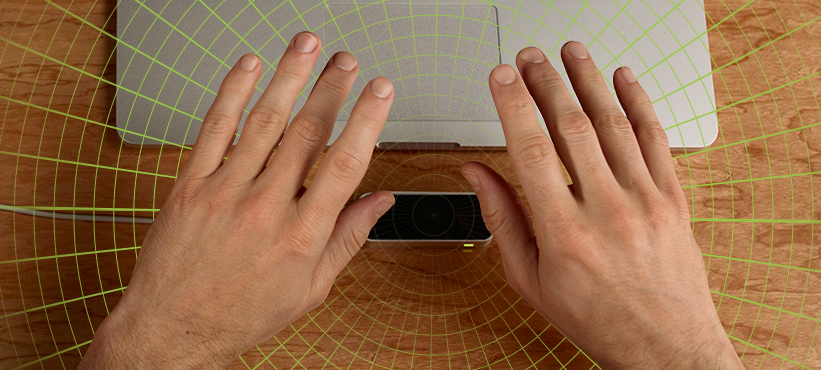
\includegraphics[width=0.3\textwidth]{leap}
         \caption{Leap Motion}
         \label{fig:leap}
      \end{figure}
En la documentación del Leap Motion  (ver figura
\ref{fig:leap}), se indica que: ``El sistema de Leap Motion detecta y rastrea
las manos, los dedos y las herramientas en forma de dedos. El dispositivo opera
en una proximidad íntima con alta precisión y de seguimiento velocidad de
fotogramas. El software de Leap Motion analiza los objetos observados en el
campo de visión del dispositivo. Reconoce las manos, los dedos y las
herramientas, y presenta información de posiciones, gestos y movimiento. El
campo de visión del Leap Motion es una pirámide invertida centrada en el
dispositivo. El alcance efectivo se extiende desde aproximadamente 25 a 600
milímetros por encima del dispositivo.'' Es importante agregar que este es
un dispositivo de bajo costo, cercano a los 100\$.

Se cuenta con acceso libre a las bibliotecas (pre-compiladas) para Linux, Mac y
Windows, para lenguajes como Python, C++ y Java. Estas identifican varios
elementos obtenidos del dispositivo: manos, dedos y herramientas y gestos.
Puede reconocer más de dos manos por captura y asociada a cada mano una lista
de dedos y herramientas. Los dedos tienen características como posición de la
punta, posición de la base y dirección en la que la punta está siendo dirigida.
En cuanto a los gestos tiene programado internamente el reconocimiento de
``círculo'' (cuando un dedo dibuja un círculo), ``swipe'' (un movimiento largo
y lineal con un dedo) y ``key tap'' y ``screen tap'' (un movimiento similar al
presionar un botón en el ratón)\\

\subsection{Emotiv}
\label{subsec:emotiv}
      \begin{figure}[ht]
         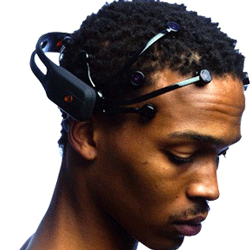
\includegraphics[width=0.3\textwidth]{emotiv}
         \caption{Emotiv}
         \label{fig:emotiv}
      \end{figure}
En la documentación del Emotiv (ver figura \ref{fig:emotiv}),
se indica que: ``Sobre la base de los últimos avances en tecnología neuronal,
Emotiv presenta una interfaz personal revolucionaria para la interacción 
persona-ordenador. Emotiv EPOC es un dispositivo de captura de señales
neuronales inalámbrico de alta resolución y multi-canal. La EPOC utiliza un
conjunto de 14 sensores y 2 referencias a sintonizar las señales eléctricas
producidas por el cerebro para detectar los pensamientos, los sentimientos y las
expresiones de los usuarios en tiempo real. La EPOC se conecta de forma
inalámbrica a PCs con Windows, Linux o Mac OS X.''

Las bibliotecas para desarrollar en Emotiv son de licencia propietaria y tienen
un valor de 201\$, adicionales a los 299\$ del equipo de hardware. La licencia
cubre la instalación en un computador. Sin embargo se encuentra a disposición
una aplicación gratis que ayuda a colocar correctamente cada sensor para
obtener las señales e interfaces para la detección de gestos faciales y para
entrenar patrones de pensamiento que desencadenan funciones en el computador.
Las dos últimas características permiten el envío de eventos de teclado cuando
se detecta una acción.

\section{Solución planteada}
\subsection{Decisiones tomadas sobre los dispositivos usados}
\label{subsec:decisiones}
El primer problema a solucionar es la elección del equipo que se va a utilizar.
Esto incluye el modelo de mano robótica, el microcontrolador que se encargue de
los movimientos y los motores para cada dedo.

Se realizó una investigación y las opciones para las manos se redujeron a dos.
El cuadro \ref{tab:manos} muestra una comparación de dos modelos. Donde se
elige la versión impresa en 3D, ya que presenta mayor impacto visual
positivo y existe todo un proyecto detrás del creador del modelado. Se han
construido más de 50, esto asegura que el producto es de calidad asegurada.

El modelo 3D nace de un proyecto de Langevin que explica
\cite{langevin_inmoov_????} como: ``InMoov es el primer robot de tamaño
natural impreso en  Open Source 3D. Replicable en cualquier impresora 3D en casa
con una superficie 12x12x12cm, se concibe como una plateforma de desarrolla de
Universidades, Laboratorios y aficionados. 
El concepto se  basa en el compartir y en la comunidad,  y le ha dado el honor
de ser reproducido para innumerables proyectos en todo el mundo.``

   \begin{table}[ht]
      \caption{Características de dos posibles manos}
      \centering
      \begin{tabular}{l c c}
      \hline
            & Cadenas de bicicleta & Impresa\\
      \hline      
            Imagen &  
\raisebox{-\totalheight}{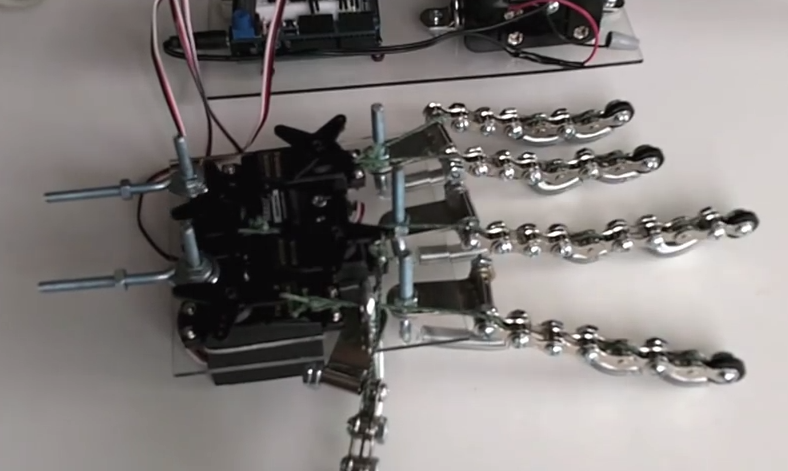
\includegraphics[width=0.12\textwidth]{manoBici}
}   &
\raisebox{-\totalheight}{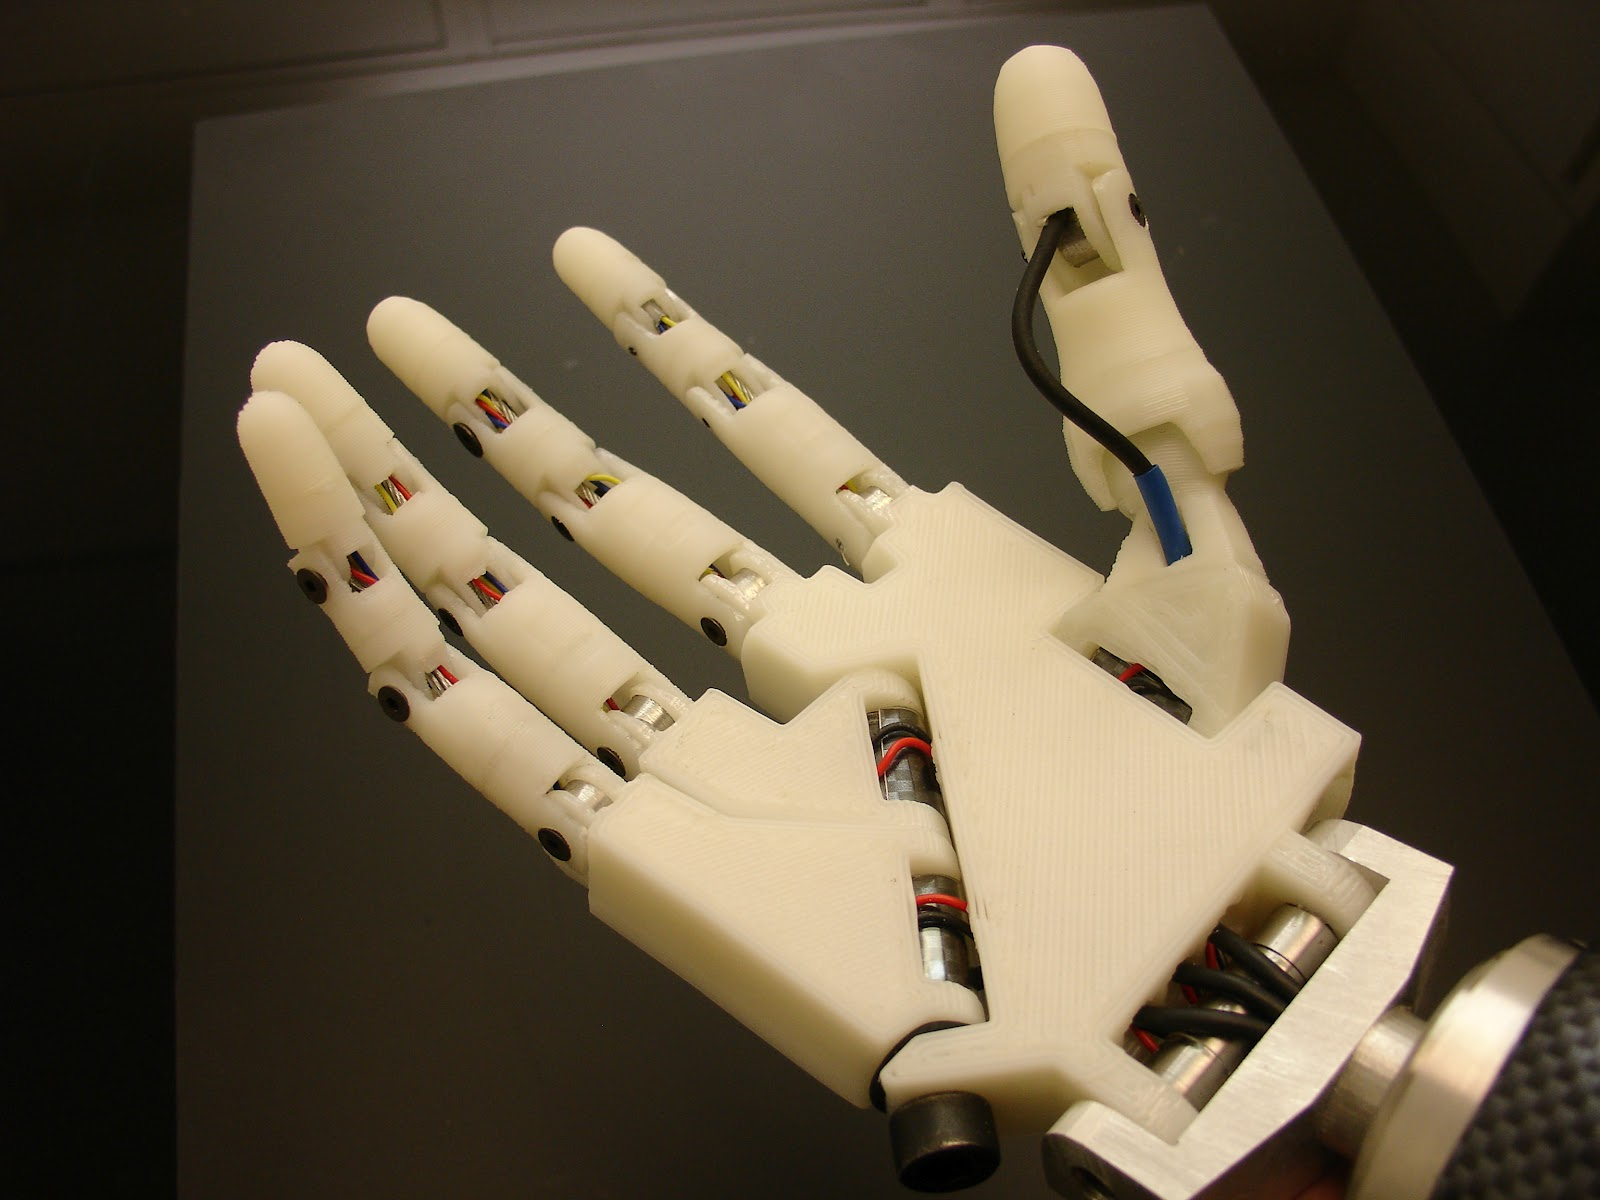
\includegraphics[width=0.12\textwidth]{manoImpresa.jpg}
}
\\
Dificultad de ensamble & Proceso artesanal & Proceso automatizado
\\
Costo & Cerca de 200\$ & Cerca de 200\$ \\
Riesgos/Beneficios & Ensamble no funciona & Resultado asegurado \\
& No encontrar piezas & Calidad impresora 3D\\
& Impacto visual & \\
         \hline
               \end{tabular}
      \label{tab:manos}
   \end{table}   
   
En cuanto al microcontrolador se toma la decisión de utilizar Arduinos. Dentro
del equipo que se tiene en el Centro de Investigación de Computación donde se
desarrolla el proyecto hay disponibles plataformas de este tipo. Estos son de
fácil programación y cuentan con los recursos suficientes para el proyecto.  Lo
que se busca en estos microcontroladores es que dispongan de al menos cinco
pines para el control de los servos, estos requieren funcionar como PWM. El
Arduino los tiene y además cuenta con una biblioteca especializada en el manejo
de servos.

Se investiga también acerca de las opciones para los motores. El cuadro
\ref{tab:servos} resume las características de tres modelos. Todas las opciones
presentan características similares, teniendo el mayor torque el MG995 y el
HK15298, sin embargo el primero se encuentra disponible en el país. Por esta
razón se utilizó este.
   
      \begin{table}[ht]
      \caption{Características de tres modelos de servos}
      \centering
      \begin{tabular}{l c c c}
      \hline
            & HK15298 & MG995 &FS5106B\\
      \hline      
         
   Tamaño [mm] & 42x20x39 & 40x20x 36.5 &40.8x20.1x38 \\
   Peso [g] & 66 &62 & 40\\
   Torque & 14kg (6v) & 15kg (6V) & 5kg(4.8v)\\

   Velocidad[s/°] & 0.13/60 (6v)& 0.13/60 (6V) &0.16/6(6V) \\
   Tension & 4.8V-7.4V & 4.8V-7.2V & 7.8-6 V \\
   Rotacion & 90° &180°&180°\\
   Precio &?? &\$15 &\$13 \\
   Comercio & ?? & crcibernetica & sparkfun\\
         \hline
               \end{tabular}
      \label{tab:servos}
   \end{table}   
   
   
\subsection{Implementación de software}
Se tomó la decisión de realizar el programa de control en C++, utilizando las
bibliotecas de Qt 4.8. Ambos sensores tienen bibliotecas en este lenguaje y
existe experiencia en el manejo del mismo. El programa cuenta con tres módulos
principales dependiendo de la plataforma de control a usar: control manual,
control con Leap Motion y control con el Emotiv. En una capa adicional se
abstraen los protocolos de comunicación, se implementa el protocolo UART
(serial) pero se deja una interfaz lista para agregar otros. Luego se programa
en Arduino un receptor de UART y se asignan cinco pines encargados de PWM para
controlar los motores responsables del movimiento de cada dedo. A continuación
se detallan los módulos, el programa en Arduino y la capa de comunicación. La
figura \ref{fig:arquitectura} resume esta arquitectura.\\
      \begin{figure}[ht]
         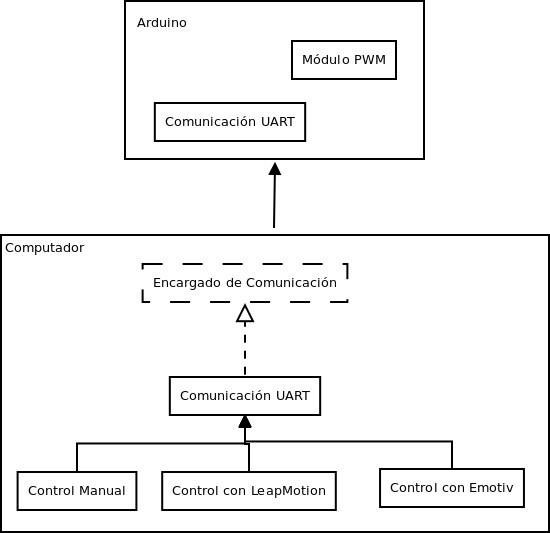
\includegraphics[width=0.5\textwidth]{Arquitectura}
         \caption{Arquitectura}
         \label{fig:arquitectura}
      \end{figure}
\subsubsection{Control manual}
Aun cuando este control no es parte de los alcances del proyecto se decide
incluir un módulo que pueda realizar fácilmente llamadas a las funciones de
movimiento desde una interfaz gráfica de usuario. Esto facilita el desarrollo
de pruebas y no deja el sistema inutilizable en caso de no disponer de los
dispositivos específicos. Se cuenta con controles deslizables, uno por cada
dedo, donde se elige fácilmente la posición a la que se desea llevar a un dedo
en específico.\\

\subsubsection{Control con Leap Motion}
La versión 1 del SDK de Leap Motion no tiene un identificador permanente para
cada dedo. Esto implica que si la mano se ve ocultada parcialmente es posible
que se pierda el control sobre el identificador de un dedo y cuando este vuelve
a foco le sea asignado uno distinto. Además, no existe manera integrada de
reconocer cual de los cinco dedos de la mano corresponde a cual, por ejemplo no
se determina si el dedo identificado es el índice o el meñique.

Para resolver esta situación se plantea implementar una función que ordena la
lista de dedos con base en su posición. De esta manera es fácil identificar
de cual dedo se trata basándose en su posición en el arreglo. En caso de
perdida parcial del foco de la mano, se activa una bandera que indica la
situación y cuando reingresa al foco se revisa el arreglo de dedos y realiza la
corrección.

El programa se basa en la posición de la punta de cada dedo para enviar las
señales necesarias a la mano sobre cuanto debe mover el dedo robot. Sin
embargo, las coordenadas se dan relativas al origen del leap motion. Es
necesario entonces realizar un cambio de coordenadas. La transformación hace
uso de las coordenadas de la mano para usar esta como origen. Así se obtiene la
misma respuesta de cambio de posición de un dedo sin importar la lejanía con el
sensor.\\

\subsubsection{Control con Emotiv}
No fue posible por parte del Centro de Investigación en Computación de adquirir
el SDK del Emotiv. Sin embargo esto no fue un impedimento para realizar un
controlador con esta plataforma. La solución planteada consistió en hacer uso
del programa llamado \emph{Control Panel} que dispone las herramientas
necesarias para reconocer señales enviadas desde el Emotiv y generar salidas
suficientes para abrir o cerrar la mano.

Los problemas con esta plataforma es la dificultad de su utilización. Como se
señaló anteriormente el dispositivo cuenta con 14 sensores y 2 referencias. La
primera dificultad es la correcta colocación. El \emph{Control Panel} en su
primera pantalla tiene indicadores para cada sensor y es necesario que cada uno
se encuentre colocado en la posición correcta y que haya sido previamente
humectado adecuadamente. Una vez colocado, existen varias maneras de procesar
las señales: gestos faciales y por entrenamiento.

El caso de los gestos faciales es de uso directo. De inmediato se puede
utilizar y genera resultados del movimiento de los ojos, de las
cejas y de la boca. Por entrenamiento es un poco más complejo de utilizar.
Primero se solicita entrenar el estado por defecto, esto es la mente en su
estado natural. Luego se pueden agregar hasta cuatro acciones que se deben
entrenar. Durante ocho segundos es necesario concentrarse en una acción para
que el sistema reconozca el patrón de señales que se genera en este estado. Lo
que resta es lograr repetir esas señales y el sistema genera una salida
distinta para cada una al reconocerlas nuevamente.\\

\subsubsection{Capa de comunicación}
Se eligió el protocolo UART y se estableció un mecanismo de comunicación para
utilizar las señales generadas por los módulos anteriores para mover cada dedo.
Se requieren dos componentes para mover un dedo: saber cual dedo mover y saber
cuanto moverlo. Los dedos se identifican con números desde el cero hasta el 4 y
es el primer mensaje enviado, seguido de un caracter de cambio de línea.
Seguidamente se envía un valor en el rango de cero y noventa dependiendo de que
tanto se desea abrir o cerrar cada dedo.\\

\subsubsection{Programa en Arduino}
Se utiliza la biblioteca de servos que dispone esta plataforma y se escribe una
función responsable de escuchar el puerto serie por donde se indica las
acciones a tomar. La biblioteca \emph{Servo.h} tiene dos funciones principales:
\emph{attach} y \emph{write}. La primera se encarga de configurar un pin del
arduino para que funcione en modo PWM y la segunda escribe valores que van a
ser interpretados en PWM. Luego se realizan las conexiones de acuerdo con la
figura \ref{fig:arduino}\\
      \begin{figure}[ht]
         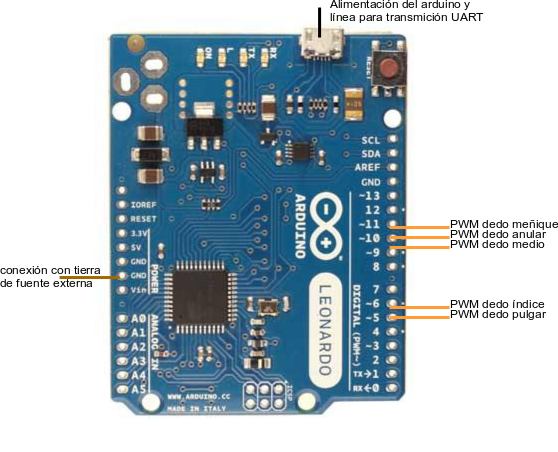
\includegraphics[width=0.5\textwidth]{arduino}
         \caption{Conexiones del arduino}
         \label{fig:arduino}
      \end{figure}

\section{Resultados obtenidos}
Se obtuvo la colaboración de la escuela de Ingeniería en Diseño Industrial para
la impresión de la mano. En esta escuela disponen de una impresora \emph{Cube}
\cite{_cubify_????}, que a pesar de no ser alta calidad es suficiente para
obtener un acabado resistente (ver figura \ref{fig:mano}). Se completa colocando
hilos de nylon como
tendones, conectados según las especificaciones de Langevin
\cite{langevin_inmoov_????}. Los servos se conectan al Arduino en los pines PWM
disponibles para este fin y se alimentan externamente con una fuente de 6V y 2A.

      \begin{figure}[ht]
         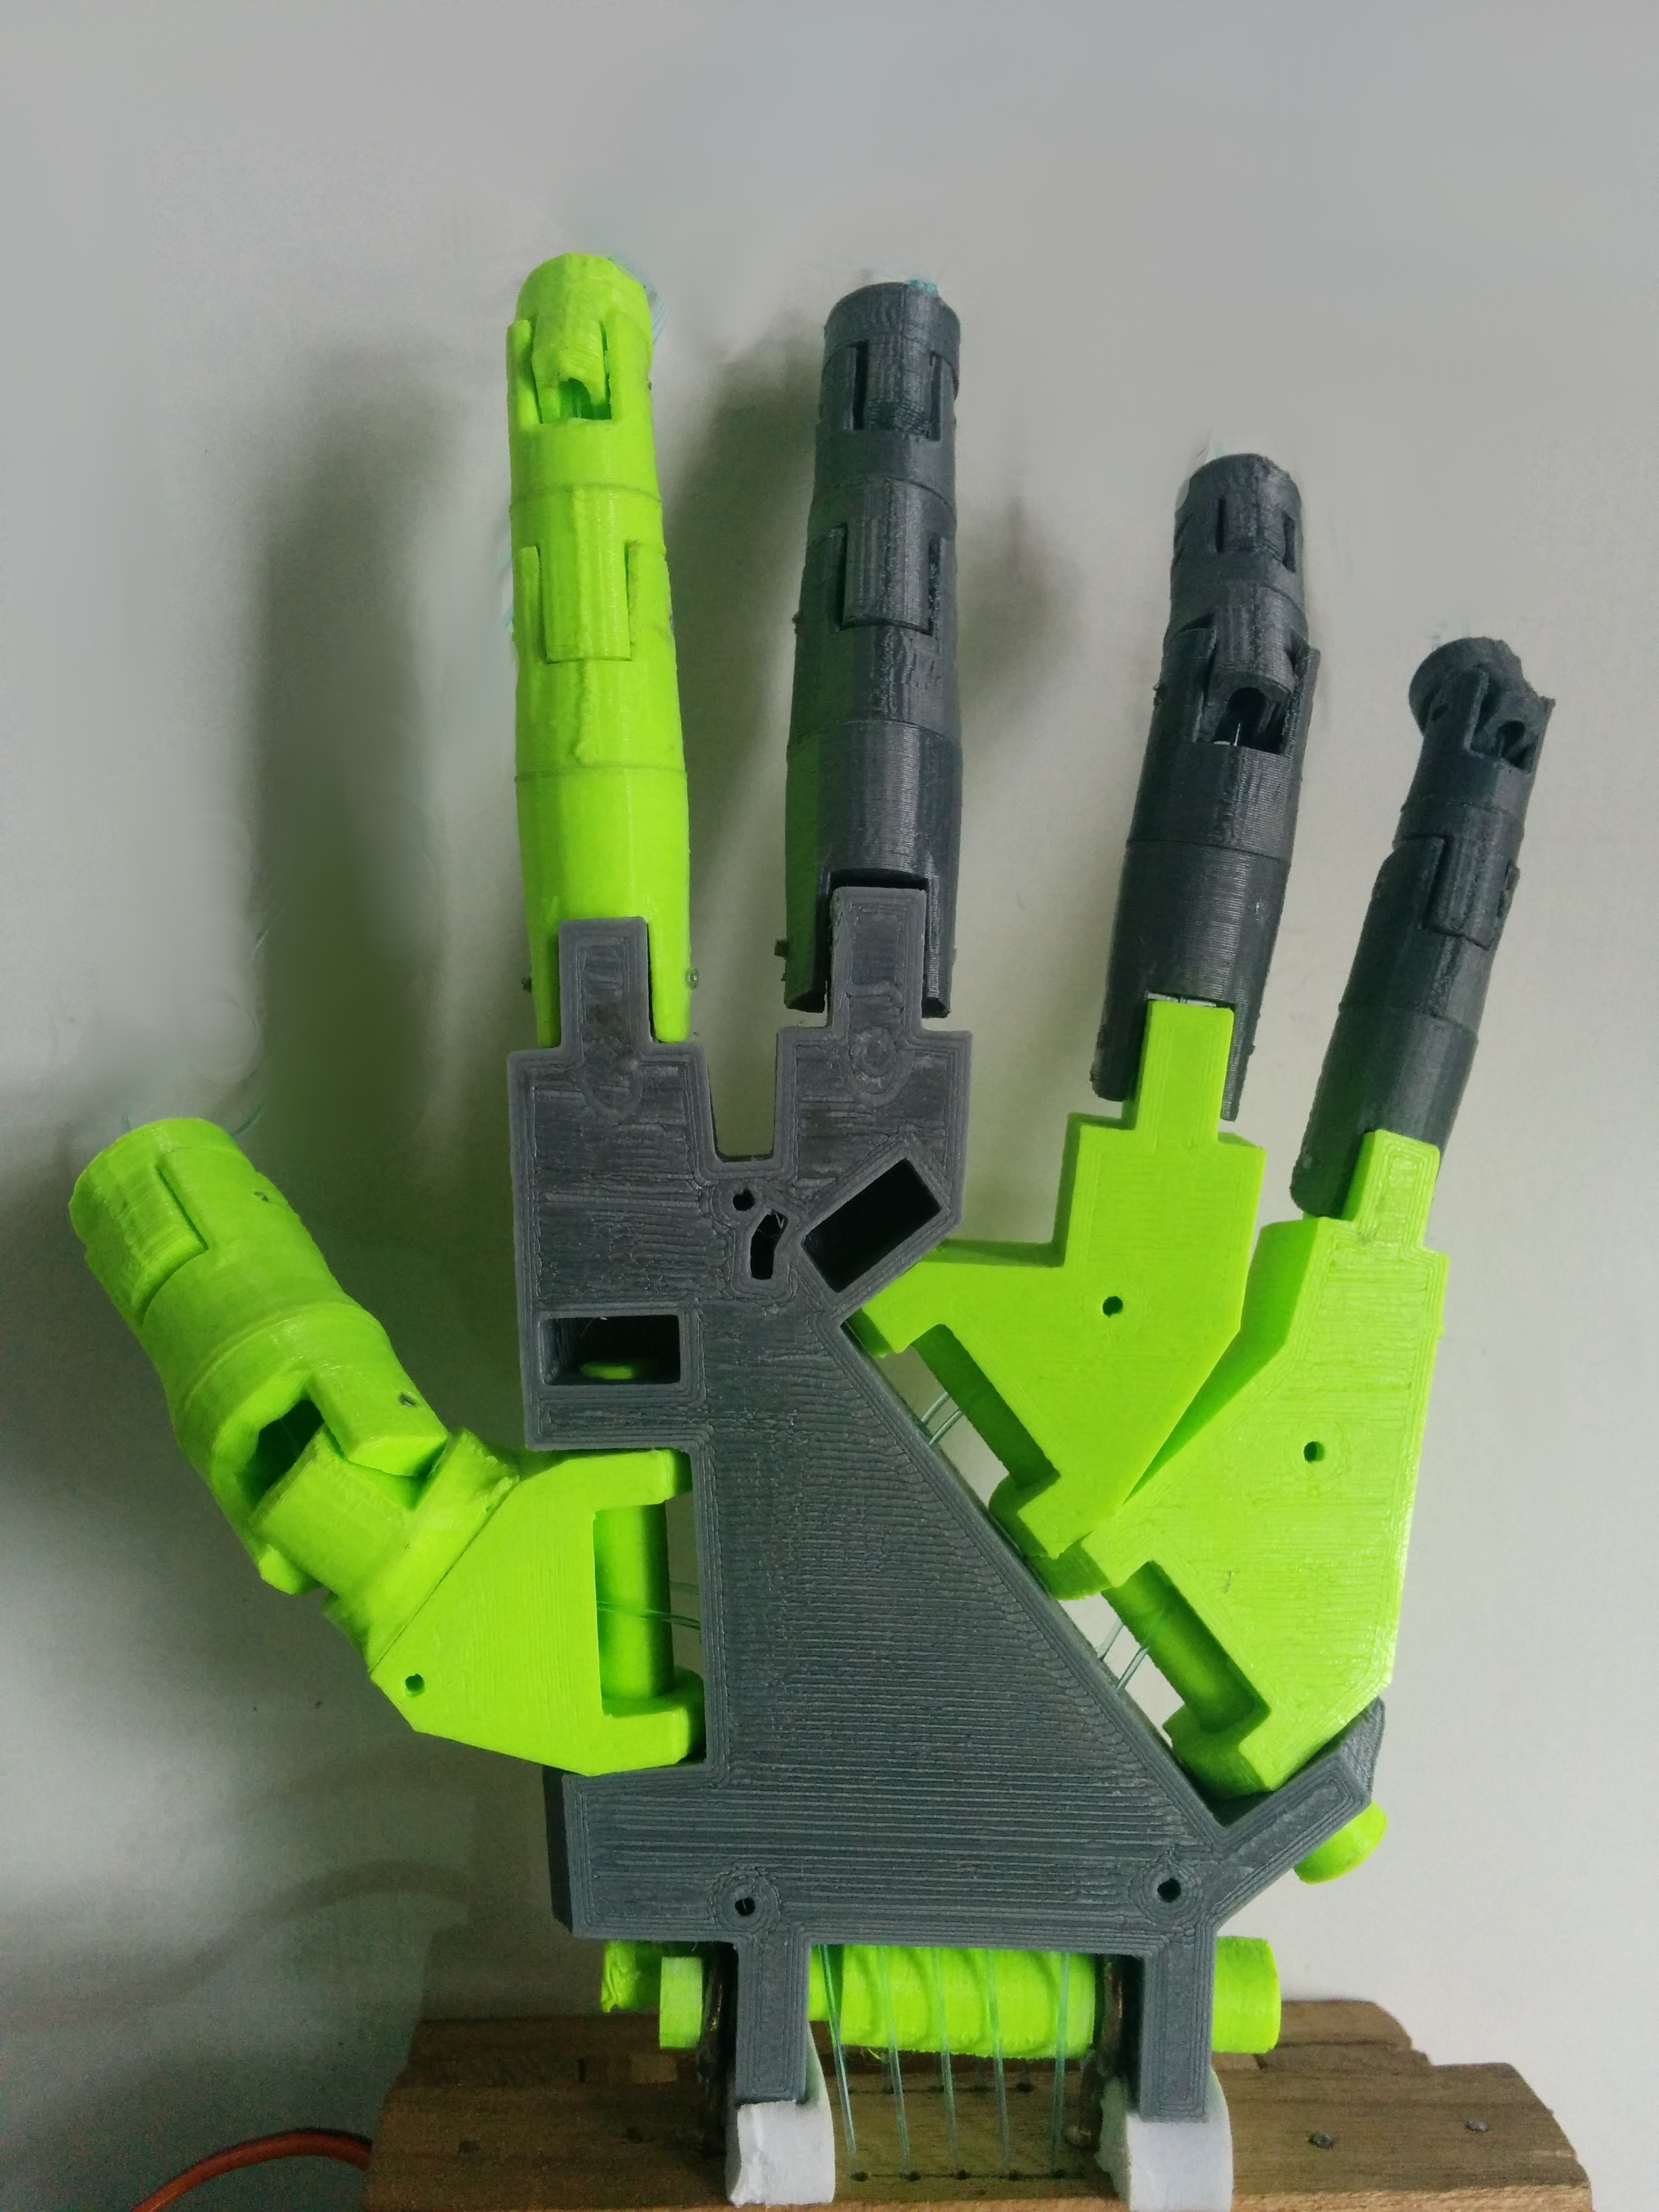
\includegraphics[width=0.35\textwidth]{mano}
         \caption{Acabado final de la mano}
         \label{fig:mano}
      \end{figure}
Para este proyecto el controlador con Emotiv se programo indirectamente
haciendo uso del \emph{Control Panel}, esto debido a que el CIC no logró hacer
la compra a tiempo del SDK. Esto provoca que se presenten dos versiones del
programa: una en Linux y otra en Windows. Solo en la de Windows se tiene acceso
a este controlador. Sin embargo la funcionalidades esperadas se cumplen y es
posible abrir y cerrar la mano robótica utilizando solo procesos mentales.

Con el Leap Motion no se presentó ningún inconveniente, e incluso se logró el
soporte en ambos sistemas operativos. El sistema detecta la presencia de una
mano dentro del rango de visión del dispositivo y envía las señales a la mano
robótica para imitar los movimientos realizados. Es posible que siga cada dedo
de la mano de manera individual y de varios simultáneamente. El gesto de cerrar
la mano totalmente también es posible.


\section{Conclusión}
Siguiendo los objetivos trazados en el plan inicial el proyecto se logra el
objetivo general, esto es se investiga y se desarrolla una mano robótica
controlable vía distintas opciones de sensores. Esto se logra basándose en el
proyecto de Langevin e investigando los API del Leap Motion y el Emotiv. 

\section{Trabajos futuros}
Al tener una mano robótica funcional y controlable desde el Leap Motion y el
Emotiv surgen nuevas ideas de proyecto que se encuentran más allá de los
alcances de este. A continuación se enlistan algunas posibilidades:
\begin{itemize}
 \item Estudiar la fuerza que la mano puede aplicar y mecanismos para
mejorarla. Esto es cuanto torque soportan los motores y cuanta tensión el
material utilizado para los tendones de los dedos.
\item Probar otros materiales para los tendones, hacer estudios de resistencia
y deformación (esto es que no se estire).
\item Establecer un mecanismo de retroalimentación para controlar la presión
necesaria para levantar o mover distintos objetos con la mano robótica.
\item Cerca del final de este proyecto los fabricantes del Leap Motion
desarrollaron una nueva versión del software con funcionalidades que vale la
pena analizar para validar si con esta se favorece de alguna manera el control.
\item Se podría validar alguna manera de utilizar de manera integrada el Leap
Motion y el Emotiv. Por ejemplo: usar el Leap Motion para entrenar movimientos
especiales y programar el Emotiv para que ejecute estos en la mano robótica.
\end{itemize}



% Can use something like this to put references on a page
% by themselves when using endfloat and the captionsoff option.
\ifCLASSOPTIONcaptionsoff
\newpage
\fi



% trigger a \newpage just before the given reference
% number - used to balance the columns on the last page
% adjust value as needed - may need to be readjusted if
% the document is modified later
%\IEEEtriggeratref{8}
% The "triggered" command can be changed if desired:
%\IEEEtriggercmd{\enlargethispage{-5in}}

% references section

% can use a bibliography generated by BibTeX as a .bbl file
% BibTeX documentation can be easily obtained at:
% http://www.ctan.org/tex-archive/biblio/bibtex/contrib/doc/
% The IEEEtran BibTeX style support page is at:
% http://www.michaelshell.org/tex/ieeetran/bibtex/
\bibliographystyle{IEEEtran}
% argument is your BibTeX string definitions and bibliography database(s)
\bibliography{bibl}



% that's all folks
\end{document}


